\section{Modeled circuits}
\label{sec:circuits}

    When thinking of which circuits to model using the analyzed EDSLs, some principles guided us.
    First of all, they shouldn't be too simple but also not too complex. Some very simple circuits
    (adders, counters, etc.) are very often shown as examples in the papers that define the EDSLs
    themselves, as well as in tutorials. On the other hand, we also did not want to model too
    complex circuits; that would require too much effort on the hardware design itself, and diverge
    from the focus of this project, which is to evaluate and analyze the EDSLs.

    Another principle that guided our choice is that the circuits should be immediately familiar to
    anyone with some minimal experience in hardware design. We avoided, therefore, considering
    application-specific circuits such as those for Digital Signal Processing (DSP), implementing
    communication protocols, etc. Having ruled out this class of circuits, we were left to choose
    from circuits that form a general-purpose computing machine, such as arithmetic units, memory
    blocks, control units and so forth.

    Finally, we wanted to choose among circuits that already had a well-defined, \emph{behavioural}
    description, to avoid using any of the analyzed EDSLs as ``basis'' of comparison.

    Taking these considerations into account, we chose to implement, in each of the EDSLs analyzed,
    three circuits originating from the book ``The Elements of Computing
    Systems''\cite{nand2tetris-book}. This book aims to give the reader a deep understanding of how
    computer systems work by taking a hands-on approach, in which the reader is given the most basic
    logic gates and builds, step-by-step, all the hardware and software components necessary to
    implement a complete computer system.

    From the hardware design part of the book, we took our three circuits to be modeled:

    \begin{itemize}
        \item A simple Arithmetic Logic Unit (ALU), from here onwards referred to as ``circuit 1''.

        \item A RAM memory block with 64 words, from here onwards referred to as ``circuit 2''.

        \item A CPU with an extremely reduced instruction set (capable of executing the \emph{Hack}
            assembly language defined in the book) from here onwards referred to as ``circuit 3''.
    \end{itemize}

    \subsection{Circuit 1: ALU}
    \label{subsec:circuit-alu}

        The Arithmetic Logic Unit built by us is a 2-input ALU, in which each of the inputs (as well
        as the output) is a 16-bit long word (interpreted as two's-complement signed integer). It is
        capable of computing several functions, and the choice of which function to compute is made
        by setting the ALU's 6 \emph{control bits}. To become more familiar with this circuit, let's
        first take a look at its block diagram, shown in figure \ref{fig:alu-block}

        \begin{figure}[h!]
            \centerline{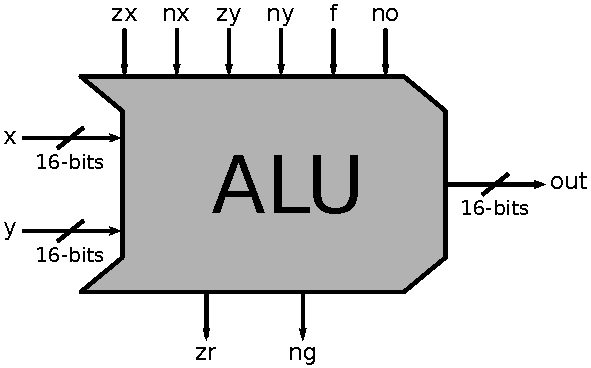
\includegraphics[width=0.5\textwidth]{imgs/alu-block.pdf}}
            \caption{Block diagram of circuit 1, showing its input and output ports.
                \label{fig:alu-block}}
        \end{figure}

        Each of the 6 control bits to the ALU has, in isolation, a well-defined effect on the inputs
        or outputs to the ALU core. The bits \texttt{(zx, nx, zy, ny)} control ``pre-processing''
        steps for the inputs \texttt{x} and \texttt{y}, with the following behaviour:

        \begin{description}
            \item[zx and zy] \emph{Zeroes} the x input (respectively y). The ALU core will receive
                \texttt{0} as input.

            \item[nx and ny] Performs \emph{bitwise negation} of input x (respectively y).
        \end{description}

        Therefore, the ALU ``core'' itself (adder, and gate) has, as inputs, the results of
        performing these pre-processing steps controlled by \texttt{(zx, nx, zy, ny)}.  Furthermore,
        the \emph{output} of the ALU core can also be \emph{bitwise negated} as a
        ``post-processing'' step, controlled by bit \texttt{no}.

        Finally, the control bit $f$ can be used to select which operation is to be performed by the
        ALU core: if we wish to add the two inputs, we need to set $f = 1$, and if we want bitwise
        conjunction, then we need to set $f = 0$.

        Besides the main (16-bit wide) output of the ALU, there are two other output \emph{flags},
        that indicate predicates over the main output:

        \begin{description}
            \item[zr] Is high whenever $out = 0$.
            \item[ng] Is high whenever $out < 0$.
        \end{description}

        When the ALU is used in the context of a microprocessor these flags can be used, for
        example, to facilitate conditional jumps.

        Even though there are $2^{6} = 64$ possible combinations for the values of the control bits,
        only 18 of these combinations result in interesting functions -- that is because several
        combinations of control bits can be used to calculate the same function. We show these 18
        functions that the ALU can calculate on table \ref{tab:alu-functions}.
        \begin{table}[h]
    \begin{center}
        \begin{tabular}{ccccccc}
            \toprule
            \textbf{zx} & \textbf{nx} & \textbf{zy} &
            \textbf{ny} & \textbf{f} & \textbf{no} & \textbf{out=}
            \tabularnewline
            \midrule

            1  &  0  &  1  &  0  &  1  &  0  &   $0$  \\

            1  &  1  &  1  &  1  &  1  &  1  &   $1$  \\

            1  &  1  &  1  &  0  &  1  &  1  &   $-1$  \\

            0  &  0  &  1  &  1  &  0  &  0  &   $x$  \\

            1  &  1  &  0  &  0  &  0  &  0  &   $y$  \\

            0  &  0  &  1  &  1  &  0  &  1  &   $\neg x$  \\

            1  &  1  &  0  &  0  &  0  &  1  &   $\neg y$  \\

            0  &  0  &  1  &  1  &  1  &  1  &   $-x$  \\

            1  &  1  &  0  &  0  &  1  &  1  &   $-y$  \\

            0  &  1  &  1  &  1  &  1  &  1  &   $x + 1$  \\

            1  &  1  &  0  &  1  &  1  &  1  &   $y + 1$  \\

            0  &  0  &  1  &  1  &  1  &  0  &   $x - 1$  \\

            1  &  1  &  0  &  0  &  1  &  0  &   $y - 1$  \\

            0  &  0  &  0  &  0  &  1  &  0  &   $x + y$  \\

            0  &  1  &  0  &  0  &  1  &  1  &   $x - y$  \\

            0  &  0  &  0  &  1  &  1  &  1  &   $y - x$  \\

            0  &  0  &  0  &  0  &  0  &  0  &   $x \wedge y$  \\

            0  &  1  &  0  &  1  &  0  &  1  &   $x \vee y$  \\

            \bottomrule
        \end{tabular}
    \end{center}
    \label{tab:alu-functions}
    \caption{Functions that the ALU can calculate, given different settings of the control bits}
\end{table}


        %% TODO: Talk about the construction of the ALU in terms of its parts.


    \subsection{Circuit 2: RAM64}
    \label{subsec:ram-circuit}

        Circuit 2 is a block of RAM with 64 lines, in which each line is a 16-bit word.  Actually,
        using the term ``RAM'' to refer to this component is an abuse of terminology, as this
        circuit is nothing more than a register bank.

        All the input and output ports of the circuit are pictured in its block diagram, shown
        in figure \ref{fig:ram-block}.

        \begin{figure}[h!]
            \centerline{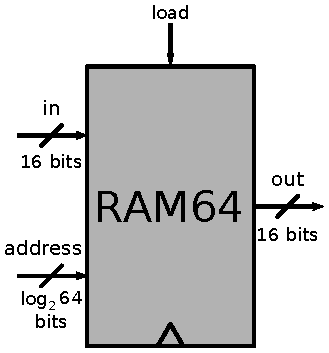
\includegraphics[width=0.3\textwidth]{imgs/ram-block.pdf}}
            \caption{Block diagram of circuit 2, a RAM of 64 lines
                \label{fig:ram-block}}
        \end{figure}

        The circuit has one 16-bit output, named \texttt{out}, and three inputs (\texttt{in},
        \texttt{address} and \texttt{load}). The \texttt{in} port is 16-bit wide and holds a value
        to be written into the RAM. The \texttt{address} port has a width of $\log_{2} 64 = 6$ bits
        and holds the address in which reading or writing is to be performed. Finally, the
        \texttt{load} bit controls whether the value currently at \texttt{in} should be written to
        the selected address. There is also one \emph{implicit} input for a clock signal in this
        component.  Implicit, in this case, means that the clock signal is not present in any of the
        models that we developed for this circuit, but must be present in any physical
        implementation.

        The temporal behaviour of this memory block is as follows: At any point in time, the output
        \texttt{out} holds the value stored at the memory location specified by \texttt{address}.
        If the \texttt{load} bit is high, then the value at \texttt{in} is loaded into the memory
        word specificied by \texttt{address}. The loaded value will then be emitted on the output at
        the \textbf{next} clock cycle.

    \subsection{Circuit 3: The Hack CPU}
    \label{subsec:hack-cpu-circuit}

        Circuit 3, the largest and most complex circuit among the ones we have chosen to implement,
        is the Central Processing Unit for the \emph{Hack} computer, the machine described in the
        book ``The Elements of Computing Systems''\cite{nand2tetris-book}.

        The Hack computer is based on the \emph{Harvard architecture}, that means that it has
        different storage components and signal pathways for instructions and data. Therefore, the
        Hack CPU expects to be connected to \emph{two} memory blocks, the instruction memory and the
        data memory. Having this in mind facilitates the understanding of the CPU's block diagram,
        shown in figure \ref{fig:cpu-block}

        \begin{figure}[H]
            \centerline{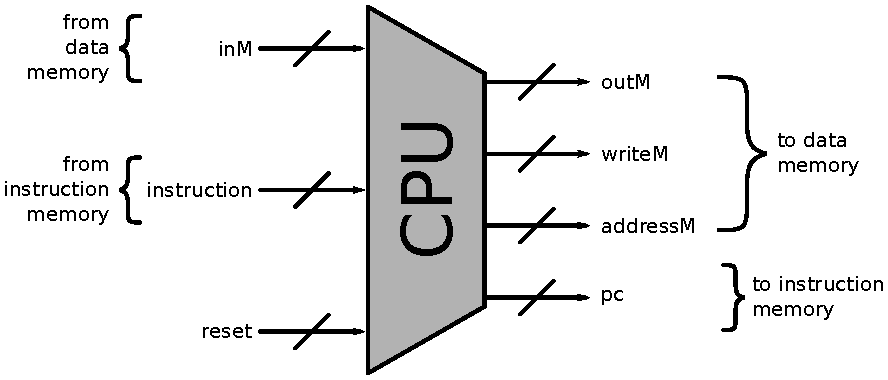
\includegraphics[width=0.85\textwidth]{imgs/cpu-block.pdf}}
            \caption{Block diagram of circuit 3, the Hack CPU
                \label{fig:cpu-block}}
        \end{figure}

        The Hack architecture has an \emph{extremely} reduced instruction set, and consists in fact
        of only two instructions (each 16-bit wide): A (meaning ``address'') and C (meaning
        ''compute''). The A instruction can be used as a means to load numerical literals into the
        data memory, as well as setting a special ``cache'' register inside the CPU. The C
        instruction is the one responsible for effectively performing computations using the ALU,
        testing outputs and jumping. More details about programming in the Hack assembly language
        can be found in \cite{nand2tetris-chapter-assembly}.

        The meaning of each of the CPU's input and output ports becomes much clearer when we look at
        the context in which the CPU is inserted, namely, the memory modules to which it is
        connected. So, let's analyze the CPU's ports by taking a look at figure
        \ref{fig:cpu-memory}.

        \begin{figure}[h!]
            \centerline{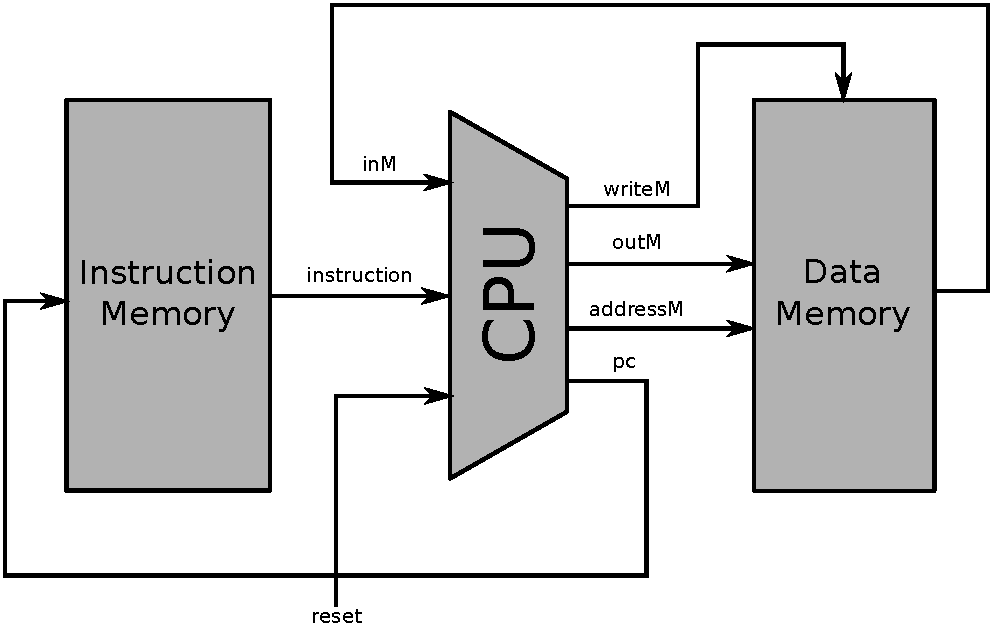
\includegraphics[width=0.85\textwidth]{imgs/cpu-memory.pdf}}
            \caption{The Hack CPU connected to the data and instruction memory blocks
                \label{fig:cpu-memory}}
        \end{figure}

        Finally, the CPU is a circuit which is built mostly from the parts we already defined in
        circuits 1 and 2. We use the ALU, some registers, multiplexers, an instruction decoder and a
        counter (the \emph{program counter}). Figure \ref{fig:cpu-parts} shows the CPU organization.

        \begin{figure}[h!]
            \centerline{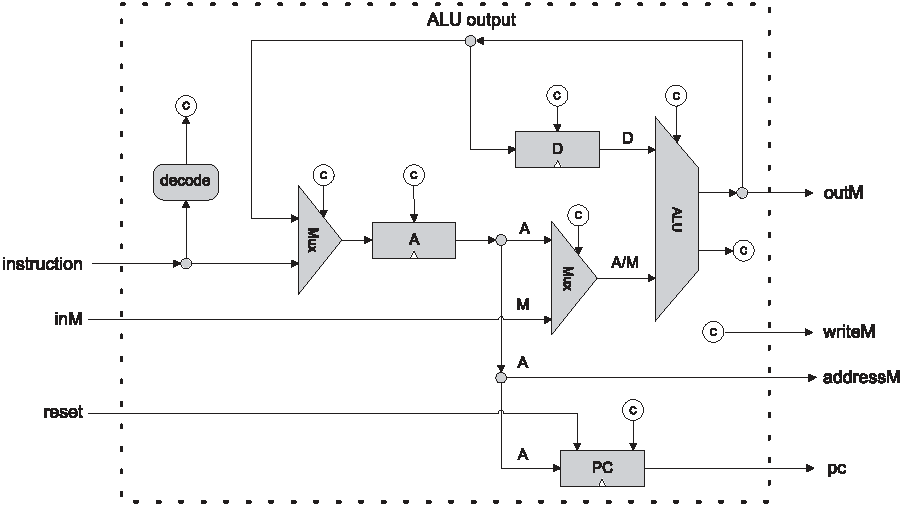
\includegraphics[width=1.0\textwidth]{imgs/cpu-parts.pdf}}
            \caption{Parts used in building the CPU circuit and how they are connected.
                \label{fig:cpu-parts}}
        \end{figure}
